% Options for packages loaded elsewhere
\PassOptionsToPackage{unicode}{hyperref}
\PassOptionsToPackage{hyphens}{url}
\PassOptionsToPackage{dvipsnames,svgnames,x11names}{xcolor}
%
\documentclass[
  letterpaper,
  DIV=11,
  numbers=noendperiod]{scrreprt}

\usepackage{amsmath,amssymb}
\usepackage{iftex}
\ifPDFTeX
  \usepackage[T1]{fontenc}
  \usepackage[utf8]{inputenc}
  \usepackage{textcomp} % provide euro and other symbols
\else % if luatex or xetex
  \usepackage{unicode-math}
  \defaultfontfeatures{Scale=MatchLowercase}
  \defaultfontfeatures[\rmfamily]{Ligatures=TeX,Scale=1}
\fi
\usepackage{lmodern}
\ifPDFTeX\else  
    % xetex/luatex font selection
\fi
% Use upquote if available, for straight quotes in verbatim environments
\IfFileExists{upquote.sty}{\usepackage{upquote}}{}
\IfFileExists{microtype.sty}{% use microtype if available
  \usepackage[]{microtype}
  \UseMicrotypeSet[protrusion]{basicmath} % disable protrusion for tt fonts
}{}
\makeatletter
\@ifundefined{KOMAClassName}{% if non-KOMA class
  \IfFileExists{parskip.sty}{%
    \usepackage{parskip}
  }{% else
    \setlength{\parindent}{0pt}
    \setlength{\parskip}{6pt plus 2pt minus 1pt}}
}{% if KOMA class
  \KOMAoptions{parskip=half}}
\makeatother
\usepackage{xcolor}
\setlength{\emergencystretch}{3em} % prevent overfull lines
\setcounter{secnumdepth}{5}
% Make \paragraph and \subparagraph free-standing
\ifx\paragraph\undefined\else
  \let\oldparagraph\paragraph
  \renewcommand{\paragraph}[1]{\oldparagraph{#1}\mbox{}}
\fi
\ifx\subparagraph\undefined\else
  \let\oldsubparagraph\subparagraph
  \renewcommand{\subparagraph}[1]{\oldsubparagraph{#1}\mbox{}}
\fi


\providecommand{\tightlist}{%
  \setlength{\itemsep}{0pt}\setlength{\parskip}{0pt}}\usepackage{longtable,booktabs,array}
\usepackage{calc} % for calculating minipage widths
% Correct order of tables after \paragraph or \subparagraph
\usepackage{etoolbox}
\makeatletter
\patchcmd\longtable{\par}{\if@noskipsec\mbox{}\fi\par}{}{}
\makeatother
% Allow footnotes in longtable head/foot
\IfFileExists{footnotehyper.sty}{\usepackage{footnotehyper}}{\usepackage{footnote}}
\makesavenoteenv{longtable}
\usepackage{graphicx}
\makeatletter
\def\maxwidth{\ifdim\Gin@nat@width>\linewidth\linewidth\else\Gin@nat@width\fi}
\def\maxheight{\ifdim\Gin@nat@height>\textheight\textheight\else\Gin@nat@height\fi}
\makeatother
% Scale images if necessary, so that they will not overflow the page
% margins by default, and it is still possible to overwrite the defaults
% using explicit options in \includegraphics[width, height, ...]{}
\setkeys{Gin}{width=\maxwidth,height=\maxheight,keepaspectratio}
% Set default figure placement to htbp
\makeatletter
\def\fps@figure{htbp}
\makeatother
% definitions for citeproc citations
\NewDocumentCommand\citeproctext{}{}
\NewDocumentCommand\citeproc{mm}{%
  \begingroup\def\citeproctext{#2}\cite{#1}\endgroup}
\makeatletter
 % allow citations to break across lines
 \let\@cite@ofmt\@firstofone
 % avoid brackets around text for \cite:
 \def\@biblabel#1{}
 \def\@cite#1#2{{#1\if@tempswa , #2\fi}}
\makeatother
\newlength{\cslhangindent}
\setlength{\cslhangindent}{1.5em}
\newlength{\csllabelwidth}
\setlength{\csllabelwidth}{3em}
\newenvironment{CSLReferences}[2] % #1 hanging-indent, #2 entry-spacing
 {\begin{list}{}{%
  \setlength{\itemindent}{0pt}
  \setlength{\leftmargin}{0pt}
  \setlength{\parsep}{0pt}
  % turn on hanging indent if param 1 is 1
  \ifodd #1
   \setlength{\leftmargin}{\cslhangindent}
   \setlength{\itemindent}{-1\cslhangindent}
  \fi
  % set entry spacing
  \setlength{\itemsep}{#2\baselineskip}}}
 {\end{list}}
\usepackage{calc}
\newcommand{\CSLBlock}[1]{\hfill\break\parbox[t]{\linewidth}{\strut\ignorespaces#1\strut}}
\newcommand{\CSLLeftMargin}[1]{\parbox[t]{\csllabelwidth}{\strut#1\strut}}
\newcommand{\CSLRightInline}[1]{\parbox[t]{\linewidth - \csllabelwidth}{\strut#1\strut}}
\newcommand{\CSLIndent}[1]{\hspace{\cslhangindent}#1}

\KOMAoption{captions}{tableheading}
\makeatletter
\@ifpackageloaded{bookmark}{}{\usepackage{bookmark}}
\makeatother
\makeatletter
\@ifpackageloaded{caption}{}{\usepackage{caption}}
\AtBeginDocument{%
\ifdefined\contentsname
  \renewcommand*\contentsname{Table of contents}
\else
  \newcommand\contentsname{Table of contents}
\fi
\ifdefined\listfigurename
  \renewcommand*\listfigurename{List of Figures}
\else
  \newcommand\listfigurename{List of Figures}
\fi
\ifdefined\listtablename
  \renewcommand*\listtablename{List of Tables}
\else
  \newcommand\listtablename{List of Tables}
\fi
\ifdefined\figurename
  \renewcommand*\figurename{Figure}
\else
  \newcommand\figurename{Figure}
\fi
\ifdefined\tablename
  \renewcommand*\tablename{Table}
\else
  \newcommand\tablename{Table}
\fi
}
\@ifpackageloaded{float}{}{\usepackage{float}}
\floatstyle{ruled}
\@ifundefined{c@chapter}{\newfloat{codelisting}{h}{lop}}{\newfloat{codelisting}{h}{lop}[chapter]}
\floatname{codelisting}{Listing}
\newcommand*\listoflistings{\listof{codelisting}{List of Listings}}
\makeatother
\makeatletter
\makeatother
\makeatletter
\@ifpackageloaded{caption}{}{\usepackage{caption}}
\@ifpackageloaded{subcaption}{}{\usepackage{subcaption}}
\makeatother
\ifLuaTeX
  \usepackage{selnolig}  % disable illegal ligatures
\fi
\usepackage{bookmark}

\IfFileExists{xurl.sty}{\usepackage{xurl}}{} % add URL line breaks if available
\urlstyle{same} % disable monospaced font for URLs
\hypersetup{
  pdftitle={Electromagnetism},
  pdfauthor={Claire Greenland},
  colorlinks=true,
  linkcolor={blue},
  filecolor={Maroon},
  citecolor={Blue},
  urlcolor={Blue},
  pdfcreator={LaTeX via pandoc}}

\title{Electromagnetism}
\author{Claire Greenland}
\date{2024-03-25}

\begin{document}
\maketitle

\renewcommand*\contentsname{Table of contents}
{
\hypersetup{linkcolor=}
\setcounter{tocdepth}{2}
\tableofcontents
}
\bookmarksetup{startatroot}

\chapter*{Preface}\label{preface}
\addcontentsline{toc}{chapter}{Preface}

\markboth{Preface}{Preface}

This is a Quarto book.

To learn more about Quarto books visit
\url{https://quarto.org/docs/books}.

Put a nice introduction here introducing the subject of electromagnetism
:D

\bookmarksetup{startatroot}

\chapter{Lecture 1: Electric Charges, Forces \&
Fields}\label{lecture-1-electric-charges-forces-fields}

\newcommand{\E}{\mathrm{\mathbf{E}}}
\newcommand{\F}{\mathrm{\mathbf{F}}}
\newcommand{\r}{\mathrm{\mathbf{r}}}

\section{Electric Charges}\label{electric-charges}

Electric charge is a fundamental property of matter. Many fundamental
particles (such as electrons and protons) have charge. However,
macroscopic objects can also be charged due to having a distribution of
charged particles on them that has a small imbalance in charge - we
might describe these as ``charged objects''.

Charge gives rise to electric fields, and hence to the electric forces
experienced between charged particles or objects.

Charge can be either a positive or negative quantity. ``Like'' charges
(charges with the same sign) repel each other, and opposite charges
attract.

Charge is quantized and comes in integer multiples of the elementary
charge \(e\) which has an approximate value of
\(1.602 \times 10 ^{-19}\) Coulombs. Electrons carry a charge of \(-e\),
and protons carry a charge of \(+e\). Charges measured in laboratories
are always multiples of \(e\) but the quarks inside protons and neutrons
and other hadrons have charges that are fractions of this elementary
charge.

Charge is conserved - or more specifically, the total charge in an
isolated system is conserved. (At least, this has been the case in all
the particle interactions physicists have so far observed.) Hence,
charge can be neither created nor destroyed, but can only be transferred
from one object to another.

\textbf{Gravitational charge:} there is one type of gravitational
charge, which is mass/energy. Gravitational charges attract. We don't
know about quantization of mass. (You can probably spend many hours on
the internet reading different opinions on this). Mass/Energy is
conserved and all everyday objects are gravitationally charged so they
all attract each other, but gravity is very weak--we can easily pick up
bits of paper with an electrically charged rod when rather few electrons
have been moved.

\section{Some definitions and important
notation}\label{some-definitions-and-important-notation}

Here I will briefly explain some notation and definitions I will use in
this course for setting up and solving problems involving electric
charges.

Consider the following ensemble of charges:

\begin{figure}[H]

{\centering 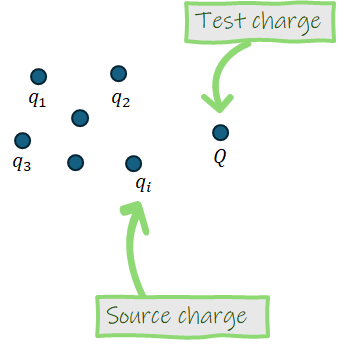
\includegraphics{Figures/sourcetest_definitions.png}

}

\caption{Some charges.}

\end{figure}%

We define the charges \(q_1\), \(q_2\), \(q_3\)\ldots{} \(q_i\) as
source charges, meaning that these are the charges that produce the
electric field for the purpose of the problem. We define \(Q\) as the
test charge, which means it is the charge that is experiencing the
effects of the electric field produced by the source charge(s). Of
course, any charge can be a source or a test charge, there is no
fundamental difference between them. ``Source'' and ``test'' are simply
names that we give charges when setting up a problem, so that we can
more easily define and solve the problem.

\begin{figure}[H]

{\centering 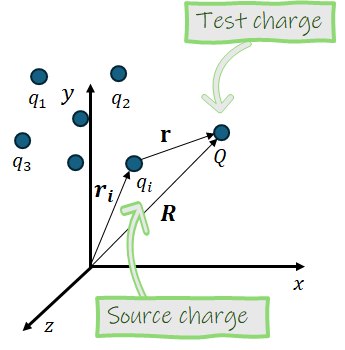
\includegraphics{Figures/axes_r_definitions.png}

}

\caption{Some charges, overlaid with axes showing the definition of
\(\mathrm{\mathbf{r}}\), the vector separation between the source and
test charges.}

\end{figure}%

\section{Electric Forces \& Coulomb's
Law}\label{electric-forces-coulombs-law}

All charges produce electric fields, and other charges that are in the
prescence of this field experience a force as a result.

The force on a test charge \(Q\), exerted by a source charge \(q\), is
given by Coulomb's Law, which is as follows:
\[ F = \frac{1}{4\pi \epsilon_0} \frac{q Q}{r^2} \hat{\mathrm{\mathbf{r}}} \]

where:

\begin{itemize}
\tightlist
\item
  \(\hat{\mathrm{\mathbf{r}}}\) is the unit vector in the direction of
  the force, which points from \(q\) to \(Q\).
\item
  \(r\) is the separation between \(q\) and \(Q\).
\item
  \(\epsilon_0\) is a physical constant known as the
  \bf{permittivity of free space}.  $\epsilon_0 \approx 8.85 \times 10^{-12}$ Fm $^{-1}$ (farads per metre). 
\end{itemize}

If \(q\) and \(Q\) have the same sign (like charges) the force is
repulsive (\(\mathrm{\mathbf{F}}\) is a positive quantity); if \(q\) and
\(Q\) have different signs, the force is attractive
(\(\mathrm{\mathbf{F}}\) is a negative quantity).

\section{Electric Field}\label{electric-field}

The vector electric field, \(\mathbf{E}\), at a particular point in
space, associated with a collection of charges, is defined in terms of
the force, \(\mathbf{F}\), exerted on a positive test charge, \(q_0\),
at that point \(E = F/q_0\).

\(\mathbf{E}\) has units of Vm\(^{-1}\) or NC\(^{-1}\). The electric
field is normally represented by field lines that indicate what a
positive test charge will do. The arrows indicate the direction of the
field and the density of lines indicates the strength of the field at a
point. The diagram shows the electric field lines for two positive point
charges of the same magnitude.

Note that the field lines are symmetric as they leave the charges. They
do not cross.

The electric field \(\mathbf{\mathrm{𝐸}}\) is a vector field that
represents the force per unit charge experienced by a positive test
charge placed at a point in space:

\[ \mathrm{\mathbf{E}}= \frac{\mathrm{\mathbf{F}}}{Q} \]

\noindent which can be rearranged to the more familiar form
\(\mathrm{\mathbf{F}}= Q \mathrm{\mathbf{E}}\). \hspace{0pt}

Electric field lines provide a visual representation of electric fields.
Key properties include:

\begin{itemize}
\tightlist
\item
  Lines begin on positive charges and end on negative charges.
\item
  The density of the lines/arrows indicates the electric field strength.
  You may also see fields drawn where the size of the arrows represents
  the electric field strength.
\item
  Lines never intersect. \hspace{0pt} \#\# Superposition Principle The
  principle of superposition states that ``the interaction between any
  two charges is completely unaffected by the presence of others''. This
  means that the total force on a test charge can be computed by
  calculating the force on the charge due to each source charge
  separately, then adding up the contributions, as follows:
\end{itemize}

\[ \mathrm{\mathbf{F}}_{tot} = \sum_i \mathrm{\mathbf{F}}_i \]

The same applies to the electric field, which can be calculated for any
given point in space as a sum of the electric field at that point from
all the source charges:
\[ \mathrm{\mathbf{E}}_{tot} = \sum_i \mathrm{\mathbf{E}}_i \]

\section{Summary}\label{summary}

Electric charges create electric fields, which exert forces on other
charges. Coulomb's Law describes the force between point charges.

\section{Bonus content: vector
fields}\label{bonus-content-vector-fields}

\subsection{What is a field?}\label{what-is-a-field}

\emph{Recommended reading:}

A field is a region of space, where property of that space is
characterized by either a number (a scalar field) or by three numbers (a
vector field).

The concept of a field circumvents the problem of action at a distance,
where one inanimate object is ``aware'' that another has arrived. We
understand that the first body sets up a field and the second body
interacts with the first via this field.

\subsection{Scalar and vector fields}\label{scalar-and-vector-fields}

A scalar field is characterized at each point by a single number.
e.g.~the temperature, \(T\), at each position in a block of metal heated
at some places and cooled at others.

\begin{figure}[H]

{\centering 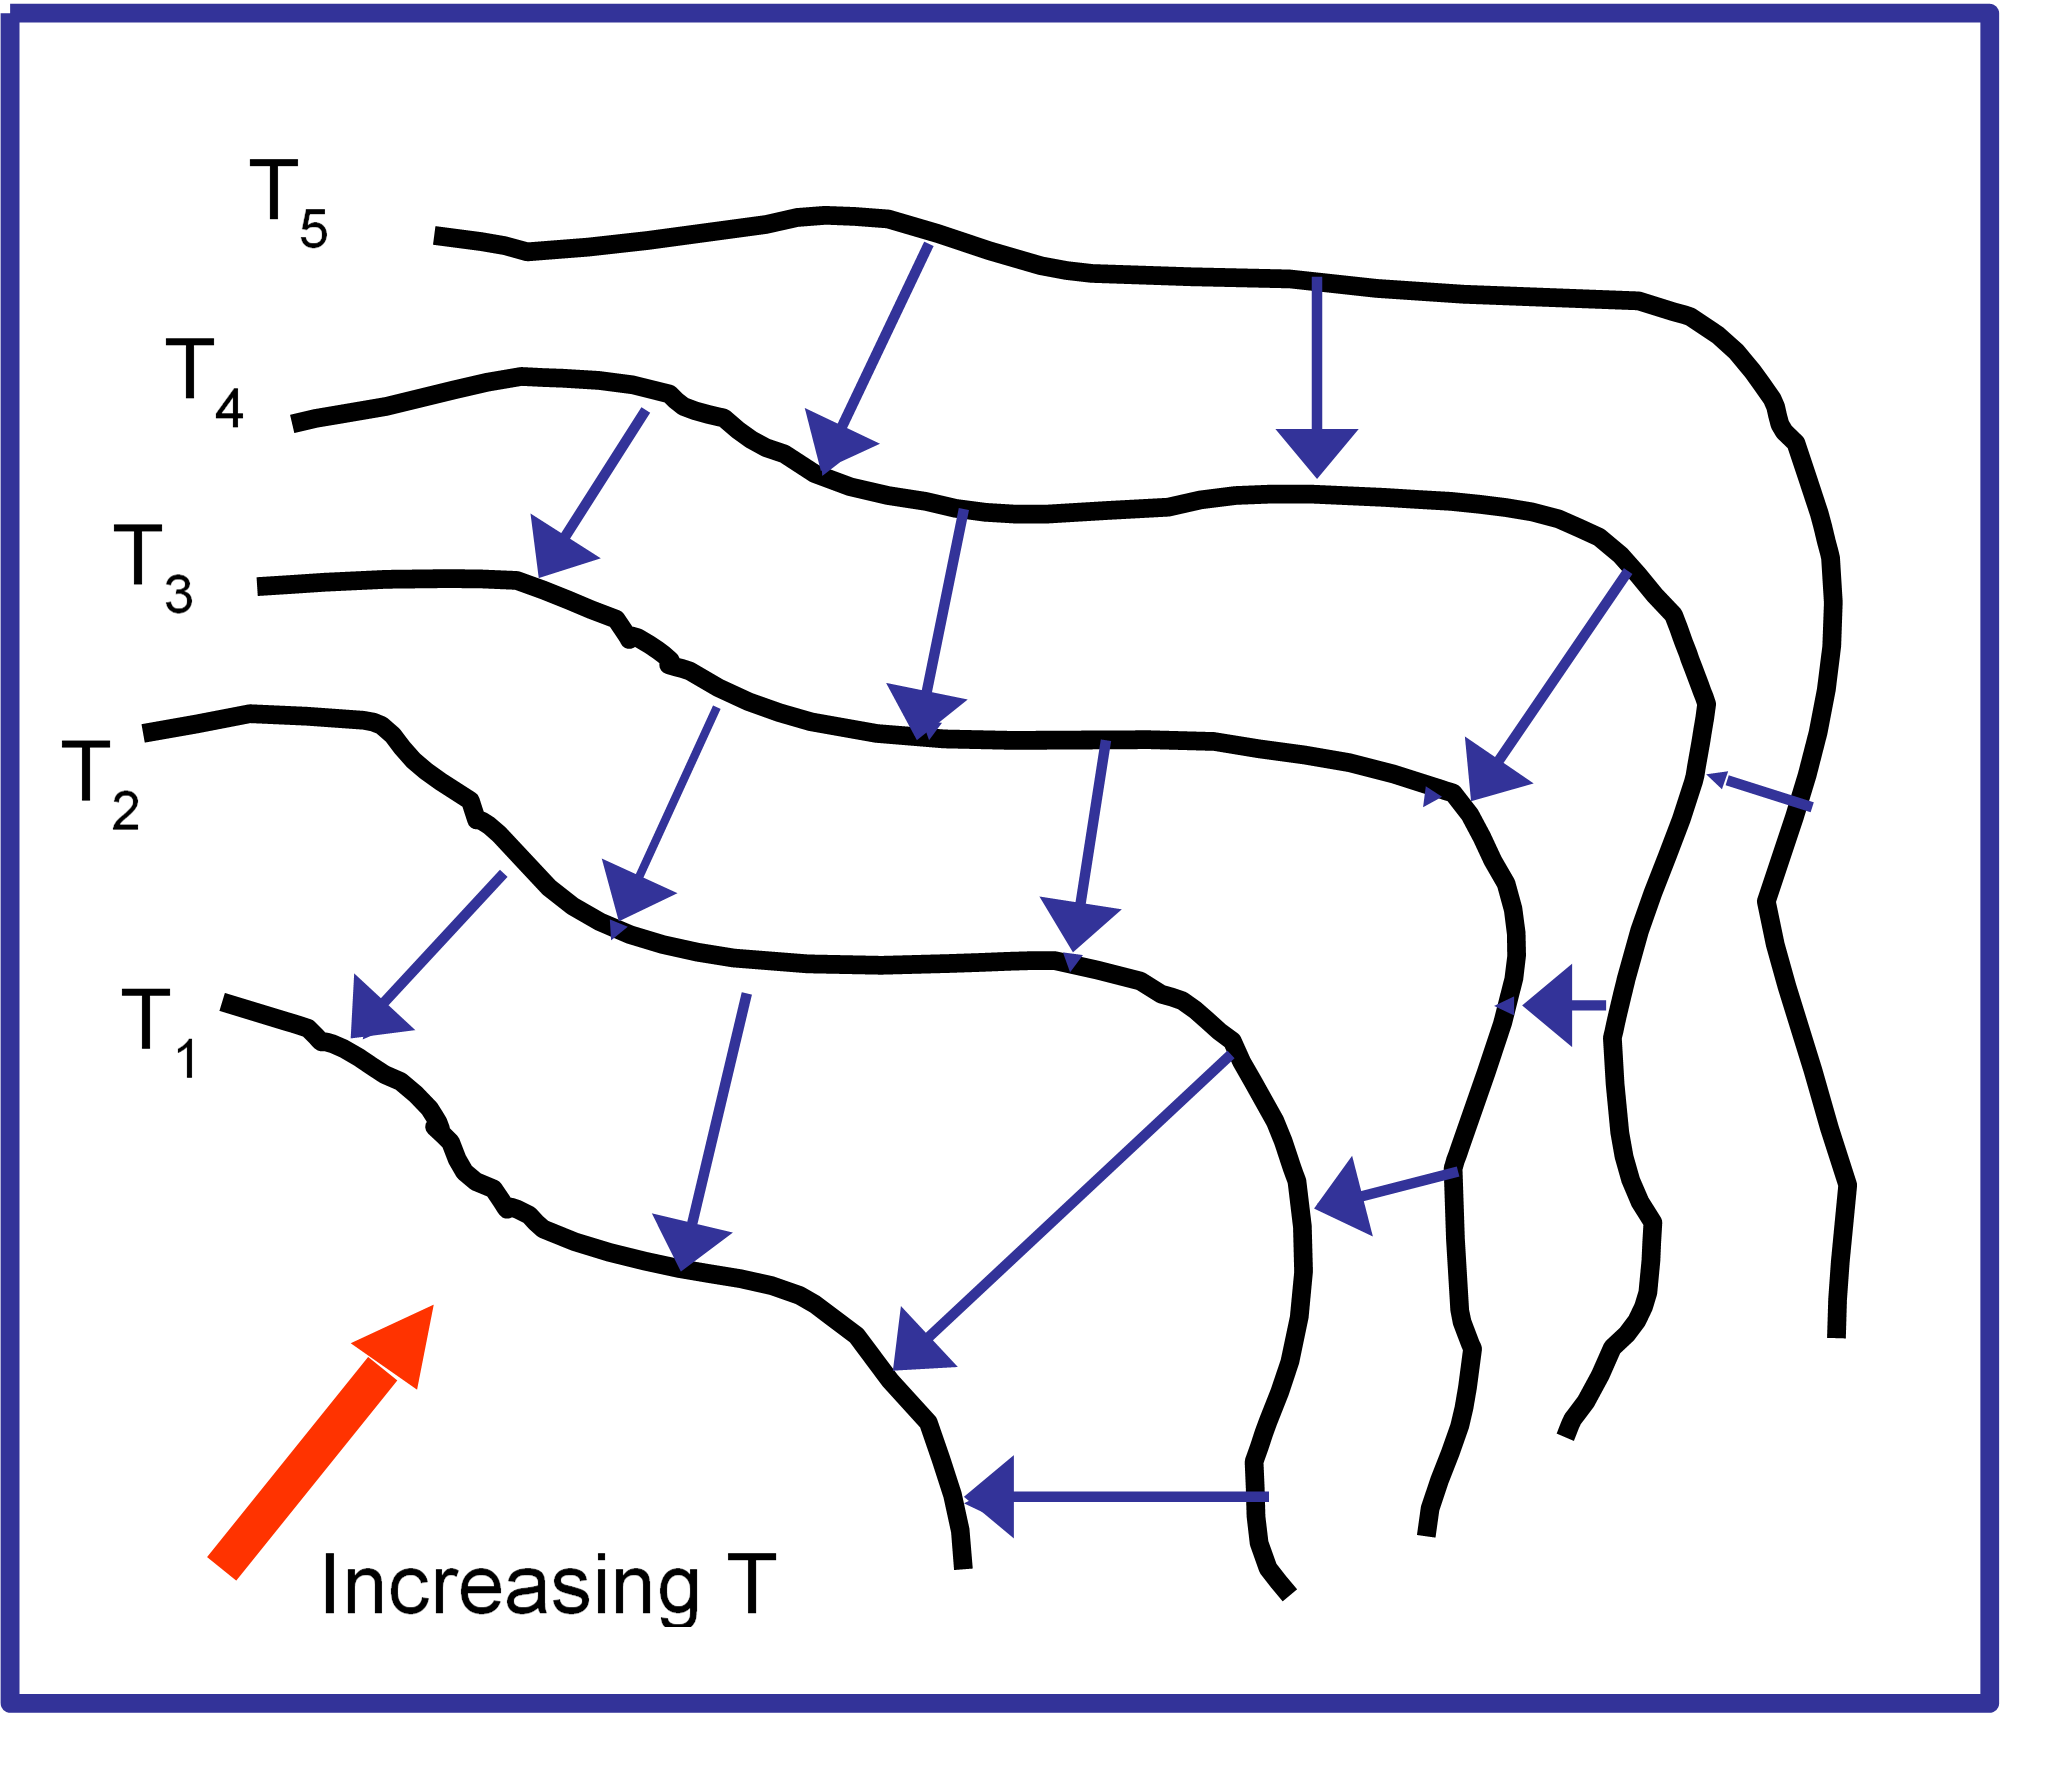
\includegraphics[width=80mm,height=\textheight]{Figures/isotherms.png}

}

\caption{A representation of a temperature field. Isotherms at different
temperatures are black lines; blue arrows show the direction of heat
flow, which is always perpendicular to the isotherms.}

\end{figure}%

\(T\) is a function of position i.e.~\(T = T(x,y,z)\). At every point we
can measure the scalar value of the temperature \(T\). The black lines
represent isotherms i.e.~lines where the temperature is constant
(\(T_1 < T_2 < T_3 < T_4 < T_5\)). Heat flow (blue arrows) is
perpendicular to the contours of constant temperature - the isotherms
(\(T_1\), \(T_2\) etc). The magnitude of the heat flow is proportional
to the temperature gradient, so that the heat flow is larger when
isotherms are closer together.

The scalar temperature field has an associated vector field, because at
any point, the heat flow is a vector, the \textbf{magnitude} and
\textbf{direction} of which depend on position. Heat flow is therefore a
vector field which is related to the scalar field of temperature. The
vector gradient of the field of heat flow depends on the temperature at
each point.

\subsection{Link between scalar and vector
field}\label{link-between-scalar-and-vector-field}

\emph{Recommended reading:}

For the scalar temperature field \(T(x,y,z)\) the vector describing the
direction and the magnitude of the maximum temperature gradient is:

\begin{equation}
 \text{Grad} \; T = \nabla T = \frac{\partial T} {\partial x} \hat{\mathbf{i}} + \frac{\partial T}{\partial y} \hat{\mathbf{j}} + \frac{\partial T}{\partial y} \hat{\mathbf{k}}
\end{equation}

The heat flow is a vector given by \(\mathbf{Q} = -k \nabla T\); the
minus sign is because heat flows from high temperature to low
temperature.

In general, for a scalar potential
\(-\nabla \phi = \frac{\partial \phi} {\partial x} \hat{\mathbf{i}} + \frac{\partial \phi}{\partial y} \hat{\mathbf{j}} + \frac{\partial \phi}{\partial y} \hat{\mathbf{k}}\)
describes the magnitude and direction of the physical effects of the
potential, with an appropriate constant if needed. In the case of the
electric field if the electric potential is \(V\) then the vector field
\(\mathbf{E} = -\nabla V\).

As an example, the gravitational field can be obtained from the
gravitational potential. The scalar gravitational potential energy is
given by \(U = mgz\) near the Earth's surface, where \(z\) is the
height. The gravitational potential is \(U/m = gz\). The gravitational
field is \(-\nabla(gz)=-g \hat{\mathbf{k}}\).

\subsection{Other operations on
vectors}\label{other-operations-on-vectors}

The vector operator \(\nabla\) behaves as a vector. We have looked at
grad \(\nabla\phi\) where \(\phi\) is a scalar field. In Maxwell's
equations, which you cover next year, you will also meet \(\nabla\)
operating on the electric field \(\mathbf{E}\):

\(\nabla \cdot \mathbf{E}\) (div or divergence)

\(\nabla \times \mathbf{E}\) (curl or rotation)

Maxwell's equations are one of the great achievements of 19th century
Physics. They link the phenomena of electricity and magnetism and can be
used to derive an expression for the speed of light. Einstein said that
the theory of Relativity was rooted in Maxwell's equations. The
equations in their differential form are shown below and we will meet
most of the concepts in this course and integral versions of some of the
laws. You can read more about Maxwell's Equations in Chapter 30 of
Tipler and Mosca.

\begin{equation}

\nabla \cdot \mathbf{E} = \frac{\rho}{\epsilon_0}
\end{equation}

\begin{equation}
\nabla \times \mathbf{E} = - \frac{\partial \mathbf{B}}{\partial t} 
\end{equation}

\begin{equation}
\nabla \cdot \mathbf{B} = 0
\end{equation}

\begin{equation}
\nabla \times \mathbf{B} = \frac{\mathbf{j}}{c^2 \epsilon_0} + \frac{1}{c^2} \frac{\partial \mathbf{E}}{\partial t}
\end{equation}

Source:
\url{http://www.clerkmaxwellfoundation.org/html/about_maxwell.html} ;
\url{https://maxwells-equations.com/}

\bookmarksetup{startatroot}

\chapter{Lecture 2: Electric
Potential}\label{lecture-2-electric-potential}

\section{Introduction to potential - relationship with electric
field}\label{introduction-to-potential---relationship-with-electric-field}

\begin{enumerate}
\def\labelenumi{\arabic{enumi}.}
\setcounter{enumi}{9}
\tightlist
\item
  Relationship Between Electric Field and Potential The electric field
  is the negative gradient of the electric potential: 𝐸 = − ∇ 𝑉 E=−∇V
\end{enumerate}

\bookmarksetup{startatroot}

\chapter{Work and Energy in
Electrostatics}\label{work-and-energy-in-electrostatics}

\bookmarksetup{startatroot}

\chapter{Magnetic Fields and the Lorentz Force
Law}\label{magnetic-fields-and-the-lorentz-force-law}

\bookmarksetup{startatroot}

\chapter{Magnetic Fields of Currents}\label{magnetic-fields-of-currents}

\bookmarksetup{startatroot}

\chapter{Magnetic Vector Potential}\label{magnetic-vector-potential}

\bookmarksetup{startatroot}

\chapter{Gauss's Law}\label{gausss-law}

\bookmarksetup{startatroot}

\chapter{Ampere's Law and Solenoids}\label{amperes-law-and-solenoids}

\bookmarksetup{startatroot}

\chapter{Faraday's Law and Lenz's Law}\label{faradays-law-and-lenzs-law}

\bookmarksetup{startatroot}

\chapter{Maxwell's Equations in Free
Space}\label{maxwells-equations-in-free-space}

\bookmarksetup{startatroot}

\chapter{Magnetisation and
Polarisation}\label{magnetisation-and-polarisation}

\bookmarksetup{startatroot}

\chapter{Maxwell's Equations in
Matter}\label{maxwells-equations-in-matter}

\bookmarksetup{startatroot}

\chapter{Capacitors and Inductors}\label{capacitors-and-inductors}

\bookmarksetup{startatroot}

\chapter{Circuits}\label{circuits}

\bookmarksetup{startatroot}

\chapter{Impedance}\label{impedance}

\bookmarksetup{startatroot}

\chapter{Summary}\label{summary-1}

In summary, this book has no content whatsoever.

\bookmarksetup{startatroot}

\chapter*{References}\label{references}
\addcontentsline{toc}{chapter}{References}

\markboth{References}{References}

\phantomsection\label{refs}
\begin{CSLReferences}{0}{1}
\end{CSLReferences}



\end{document}
